\documentclass[conference,compsoc]{IEEEtran}
% \documentclass{IEEEconf} 
\usepackage{url}
% \usepackage{hyperref}
\usepackage{amssymb,amsmath}
\usepackage{pdfpages}
\usepackage{graphicx}

% \title{No solution? Clustering to Evaluate Multiple Imputation } 
% \title{CLEMI (CLustering to Evaluate Multiple Imputation: The Framework}
\title{CLEMI: A Proof-of-Concept Computational Framework for Clustering to Evaluate Multiple Imputation}
% \author{Anthony S. Chapman, Steven Turner, Wei Pang, Lorna Aucott} 
\author{
    \IEEEauthorblockN{Anthony Chapman\IEEEauthorrefmark{1}\IEEEauthorrefmark{2},
    				  Steve Turner\IEEEauthorrefmark{3},
    				  Wei Pang\IEEEauthorrefmark{1}, 
    				  Lorna Aucott\IEEEauthorrefmark{2}}
    \\ \IEEEauthorblockA{\IEEEauthorrefmark{1}School of Natural and Computing Sciences, University of Aberdeen, UK, AB24 3UE}
    \\ \IEEEauthorblockA{\IEEEauthorrefmark{2}Institute of Applied Health Science, University of Aberdeen, UK, AB25 2ZD}
    \\ \IEEEauthorblockA{\IEEEauthorrefmark{3}Child Health, University of Aberdeen, UK, AB25 2ZG}
}

\begin{document} 
	\maketitle{} 

% Glad I could help. You already have a quarter of a paper. 
% Some initial comments:
% Personally, I would do the discussion before the conclusion, or incorporate the two together as Discussion and Conclusion. Remember - don't use colloquial language.
% Also, you want to head a section as The Problem to make it abundantly clear what it is. You need to lead them by the nose. You must always explain what you are going to tell them, tell them what you are going to tell them, then tell them what you have told them to get the message across -subtly, of course. Expand Acronyms the first time you use them. Also, explain everything if you want the paper to appeal to a wider audience. If you write for an audience who understand all the language, great for them, but if you want to refer to it later for a different audience, better to make it super clear and lead them by the hand.

% Anyway - you are off and running. Good luck - you'll have three papers in no time at all.

% There is nothing to easily compare different imputation techniques, post researches haven't got computing background... (need a way to formally say that statement, maybe number of disciplines VS computing?? ) 

	% \abstract{
	\begin{abstract}
	Data with missing values are ubiquitous across the world Although computational and statistical approaches have been developed to deal with missing values, a vast majority of researchers choose to carry out complete case analysis instead of using software to predict missing values. Our approach evaluates the effect of imputation by using clustering. To our knowledge there has not been any ongoing evaluation of imputation.

	This paper presents a framework for a system, the purpose of which, is to allow those researchers who do not have sufficient computational or statistical analysis skills to facilitate better understanding of different imputation techniques and how they affect and contribute to data analysis. In addition, it sets guidelines on how such a system can be used to choose an appropriate imputation methods. The system could also be used to optimise an imputation method by analysing the effect changing the parameters have on the dataset.
	\end{abstract}	
	% }

	\section{Introduction} % (fold)
	\label{sec:introduction}
		Researchers from all disciplines have to analyse raw data presented to them at some stage of their research. There are common problems in data analysis, for instance, organizing the data, dealing with outliers, missing values, data manipulation; just to name a few. When dealing with routinely acquired data\cite{routine}, one of the main problems a researcher faces is what to do about missing values. Multiple imputation\cite{mi} is a possible solution for missing values, although there is work on how to impute (replace missing value with a value) values, there is no  way to evaluate it's effects or efficiency. We present a way to evaluate the effect of any given imputation method and provides guidelines to make such a system accessible to all researchers regardless of their background. 

		Firstly, we describe some of the problems a researcher faces when analysing data with missing values. Secondly, we discuss possible solutions for dealing with missing data including ways to evaluate such solutions, we then outline a framework which is not language specific.

		This paper is the first attempt in an effort to create software which supports researchers in evaluating the effect of multiple imputation, regardless of their computing and statistical abilities. We finally provide some preliminary results from our implementation which is being written in R, a statistical programming language. 
	% section introduction (end)

	\section{Background} % (fold)
	\label{sec:background}

	In this section we introduce some key concepts of routinely acquired data, why missing values occurs, the current practises when dealing with missing data and some ways to analyse data with missing values. 

		\subsection{Missing Data} % (fold)
		\label{sub:missing_data}
		Our project deals with routinely acquired maternity data, like many other scientists from all disciplines\cite{bigData}, we encounter datasets with missing values. The amount of missingness in one of our datasets is as high as 85\% of all records having one or more values missing. Before any analysis can be carried out, we need to decide on the best way to analyse data with missing values. We could ignore any records with missing values and carry out the analysis on the subset consisting of all records with no missing values (complete case analysis). Additionally, we could impute missing values with predicted values.

		After searching relevant literatures, and current systematic reviews of cohort studies \cite{systematic1,systematic2,systematic3} which show how hundreds of different studies dealt with missing data. We noticed that the majority (circa 70\%) use complete case analysis, and some (circa 25\%) do not mention whether there were any missing values or what they did if there were. 

		\textcolor{red}{(Theory about most data possible for better analysis)} 

		In our case, complete cases analysis on the maternity dataset will only yield 15\% of the data. This means only 15\% of the available data could be used for analysis. Although ignoring missing values seems to be acceptable in some cases, the systematic reviews also show studies which impute missing values prior to any analysis. Imputation has been shown to be effective\cite{impact} but it should not be taken lightly, 9\% and 6\% (respectively) of the studies reviewed \cite{systematic1,systematic2} used imputation methods that are known to produce biased results\cite{mean}.

		\textcolor{red}{and depend heavily on the assumptions about the relationship of the missing data and the outcome of interest}
		taking us back to the problem that it only represents 15\% and could be biased w.r.t. any specific outcome variable
		% subsection missing_data (end)

		\subsection{Imputation} % (fold)
		\label{sub:imputation}
		We decided to use the statistical computing software R \cite{r} for the analysis as we are comfortable with the language and there is a large community for support. After deciding on the language, we chose a package called MICE \cite{mice}. While MICE seems to suit our needs, we are unsure whether this imputation method (or another) will enhance our data for better analytical results. Even if this method has been proven to work on a dataset, it does not indicate that it will work on all others. 

		Multiple imputation works by replacing each missing value with a set of plausible values that represent the uncertainty about the right value to impute. The imputed datasets are then analysed and the results are combined. Multiple imputation does not attempt to estimate each missing value through simulated values but rather to represent a random sample of the missing values. This process results in valid statistical inferences that properly reflect the uncertainty due to missing values; for example, valid confidence intervals for parameters\cite{mi}. 

		In order to check whether the imputation method works on a given dataset, one can first apply the method to a benchmark dataset and analyse the effects of such an action. For this process to imply the effects of the method on the given dataset, the benchmark must follow the same pattern of missingness as our dataset. Unfortunately, it is often difficult and time consuming to find such a benchmark. It would be almost impossible to find a benchmark which could also be used for a wide range of datasets. Thus, we felt that benchmark datasets should also be specific to the given dataset. One could create a benchmark by analysing the way values are missing in the dataset and applying it to a dataset which is complete. The best complete dataset to mimic the original behaviour could be a complete cases dataset extracted from the original dataset.
		% subsection imputation (end)
		

		\subsection{Clustering} % (fold)
		\label{sub:clustering}
		
		The next challenge will be to interpret the effect of imputing a dataset with any given imputation method. Measure theory \cite{measure} and cluster analysis \cite{clustering} provide good starting points on achieving this since measure theory will help us compare multidimensional datasets to each other and clustering can create comparable efficiency outputs from imputed datasets. Measure theory provides systematic ways in which to assign numbers to suitable members of a group, this way one can give a sense of distance in a less conventional manner (for example, what is the distance between record 5 in a dataset and the average record in the same dataset, note the dataset could include categorical variables). 

		Clustering is an unsupervised computation method which takes a group of items and puts them into smaller groups according to their characteristics. The idea being, all items that behave similarly will be put into a group

		all other items will be in other groups. Each of these groups is called a cluster and a group of clusters is called a clustering, some cluster and clustering characteristics that might be of use are the cluster sizes (amount of objects in each cluster), maximum dissimilarity (maximum distance between an object in a cluster and the cluster's centre object), average dissimilarity (the average distance between all points in a cluster and it's centre object), the average width of each cluster in a clustering and the cluster isolation values (how separated each cluster is from the other clusters)\cite{clust-char}.
		% subsection clustering (end)

	% section background (end)

	\section{The Challenges} % (fold)
	\label{sec:the_problems}
	When working with raw routinely acquired data, one of the first challenges a researcher will have to overcome is how to deal with missing values \cite{rountine-missing}. With large amounts data being collected daily \cite{bigData}, data corruption is inevitable and can happen at any point during data acquisition. These data corruptions may happen due to human error, computational inefficiency or other unforeseen circumstances \cite{reason}. Missing values in a dataset create an array of problems that need to be solved. Firstly, missing values could affect the results from any analysis. Secondly, a way to replace missing values needs to be chosen. Thirdly, one needs to confirm whether the chosen method will work on any dataset. Finally, we need to evaluate the chosen method to know whether it is the best way. We now discuss some of these challenges and provide possible solutions.

		\subsection{Incompleteness / Missing Values} % (fold)
		\label{sub:incompleteness}
			Missing values are more likely the closer you access the dataset at it's source, thus raw data will have the most missing values. Although there are ways to combat missing data, such as mean-value imputation or multiple imputation \cite{missing1,missing2,missing3}, it is still quite normal for researchers to perform complete cases analysis \cite{epi1,systematic1,systematic2,systematic3}. As an example, in \cite{epi1}, the authors use only 2,758 records for analysis out of the possible 44,261 mainly due to missing data, and this is a mere 6.2\% out of the records available.
			\subsubsection{Possible Solution: Imputation} % (fold)
			\label{sub:possible_solution}
				Imputation is the process of replacing missing values with substituted values. One has to be careful when imputing data as there are many techniques (default value, mean value and multiple imputation just to name a few \cite{gelman2007data}) and using them without care will lead to erroneous data analysis \cite{careful}. By creating a user-friendly system with clear guidelines on how to impute data and some explanation on how it works, we believe that researchers that would normally ignore data with missing values will be more likely to use more of the available data through imputation, thus improving the quality and credibly of their analysis.
			% subsection possible_solution (end)
		% subsection incompleteness (end)
		\subsection{Applicability of Imputation} % (fold)
		\label{sub:will_it_work_on_my_data}
			After deciding that imputation is beneficial to the study, the next step will be to find an imputation method for the dataset. Muliple Imputation by Chained Equations (MICE \cite{mice}) using the computational language R \cite{r} or the Impute Missing Values function in the statistical software SPSS \cite{spss} are two example of imputation which are accompanied by documentation to support them. The problem is, how does one know if the imputed values are representative to the truth, how does one know whether the imputed values are the correct values after applying the imputation method.

			Even if the imputation method has been proven to work on a specific dataset such as \cite{compare}, it is no indication it will work for any other dataset. This is due to the complex nature in which missing data is created, for example there might be a underlying reasons for the variables to be missing\cite{missing4,missing5}. 

			In order to test whether an imputation method works on other datasets, one needs something to compare the results to; a benchmark. We could the analyse the effects of imputation by comparing the effects on the benchmark. Unfortunately, it is difficult to find a complete dataset to use as a benchmark which would reflect the effects imputation will have on the original dataset.
			\subsubsection{Possible Solution: Testing one's own data} % (fold)
			\label{sub:possible_solution}
				The proposed solution is to create clone datasets by analysing the missingness characteristics from a given dataset and applying them to a new dataset created by the complete records. We can therefore create benchmark datasets which have the same characteristics as the original dataset. We now have an original dataset, a subset consisting of only the complete records (the benchmark) and artificially incomplete datasets created from the complete records with the missingness characteristics from the original. 

				We then have a benchmark and a testing dataset which behaves similar to the original dataset in terms of missing values. The idea being that if the imputation method works on the testing datasets, it will work on the original, and we can test whether imputation is successful by comparing to the benchmark. 
			% subsection possible_solution (end)
		% subsection will_it_work_on_my_data_(end)
		\subsection{Choosing the best imputation technique} % (fold)
		\label{sub:which_imputation_is_best_for_me}
			The following problem applies to researchers, even those computationally competent, who wish to know whether one imputation method is better than any others. There is nothing to easily compare results from different imputation methods or the same imputation methods with slightly different parameters. The main problem arises when one tries to compare the outcomes from one method to another, here an adequate analogy would be to compare imputation method A with method B would be like comparing chocolate with a bicycle; the outcomes might not be comparable. 

			A framework which can take different imputation methods and output scores in order to compare the effects of imputing a dataset is needed. It is essential that the framework can be implemented into a system accessible by all researchers. 

			\subsubsection{Possible Solution: Comparing Imputation} % (fold)
			\label{sub:possible_solution}
				In order for a researcher to be able to compare different imputation techniques on their own datasets, the outcomes of the techniques need to be compatible. A system that imputes a dataset and outputs a standardised efficiency classification which will make it easier to compare different imputation methods on the same dataset using this standardised efficiency classification. 

				 A program which can be used by every researcher, regardless of their computing or statistical ability, to deal with missing data would be beneficial.Thus every researcher will be able to compare different imputation methods without having to understand the individual imputation technique outputs.
			% subsection possible_solution (end)
		% subsection which_imputation_is_best_for_me (end)
	% section the_problems (end)

 

	\section{CLEMI: The Framework} % (fold)
	\label{sec:proposed_framework}
		\textbf{The idea:} The underlying concept is to first create a benchmark dataset from the complete records, then create artificially missing datasets which represent the original dataset out of the benchmark by mimicking the original dataset. We achieve this by analysing the pattern of data missing for a specific dataset and create testing datasets by imposing the same missingness into the benchmark. We would then impute the artificially missing datasets and analyse how far they have deviated from the benchmark. We can check how far imputation has taken the datasets from the benchmark by clustering the benchmark and the testing datasets. By doing so we will be able to see the effects of imputing a dataset. 
		\\
		\indent \textbf{Pre-requisite:}
		In order to evaluate the effect of applying an imputation method on a dataset, one has to first have a dataset with missing values and choose an imputation method. At this stage, any imputation method can be used to accommodate the ability to compare different imputation methods on the same dataset to evaluate the best one. Similarly, one can apply the same imputation methods to the dataset multiple times by changing the imputation parameters, thus finding the optimal imputation. We will call the dataset $O$ and imputation method $imp(x)$, where $x$ is any incomplete dataset.
		\\
		\indent \textbf{Stage 1: Extracting a Benchmark}
		Firstly, a benchmark needs to be created, this can be done by extracting the complete records from $O$; call this benchmark dataset $CC$ for Complete Cases. $O$ can then be analysed to find the missingness characteristics, this will be used to create replicas later in the process. Notice that $ CC \subset O$ 
		\begin{figure}[!ht]
			\caption{Stage 1}
			\centering
			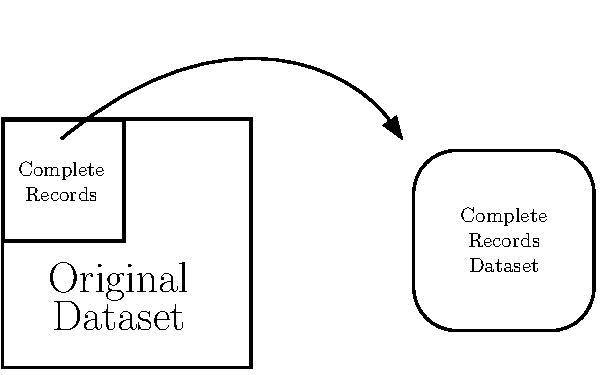
\includegraphics[width=0.35\textwidth]{stage1.pdf}
		\end{figure}
		\\
		\indent \textbf{Stage 2: Create Dummy Datasets}
		Next, artificially incomplete datasets are created, called $artMiss.i$ where $i$ is a number from 1 to $n$ by applying the missingness characteristics from $O$ to $CC$ $n$ times. It is important to apply the missingness in a manner that treats each $artMiss.i$ separately; doing so will aid in a more robust test. Thus we now have a benchmark dataset $CC$, and $n$ artificial datasets with missing data which follow the same structure as the original dataset.
		\begin{figure}[!ht]
			\caption{Stage 2}
			\centering
			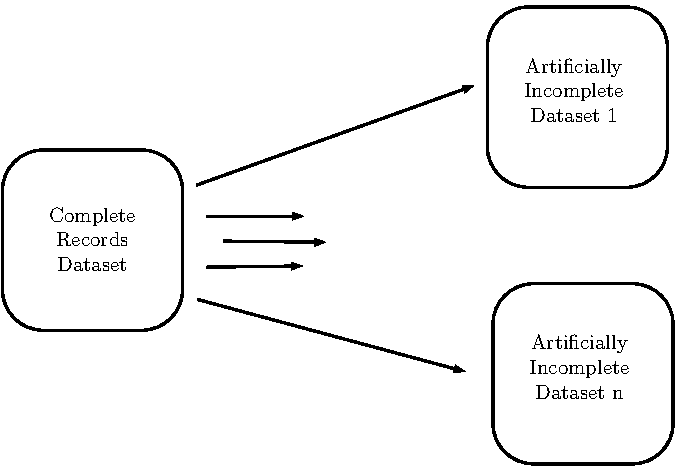
\includegraphics[width=0.35\textwidth]{stage22.pdf}
		\end{figure}
		\\
		\indent \textbf{Stage 3: Impute Dummy Datasets}
		The next step will be to impute all $artMiss.i$ with the chosen imputation method, it is important to apply exactly the same procedure (same imputation with the same parameters) to all datasets in order to have reliable results. This will create $n$ artificially complete (imputed) datasets, called $artComp.i$ where $i$ ranges from 1 to $n$. 
		\begin{figure}[!ht]
			\caption{Stage 3}
			\centering
			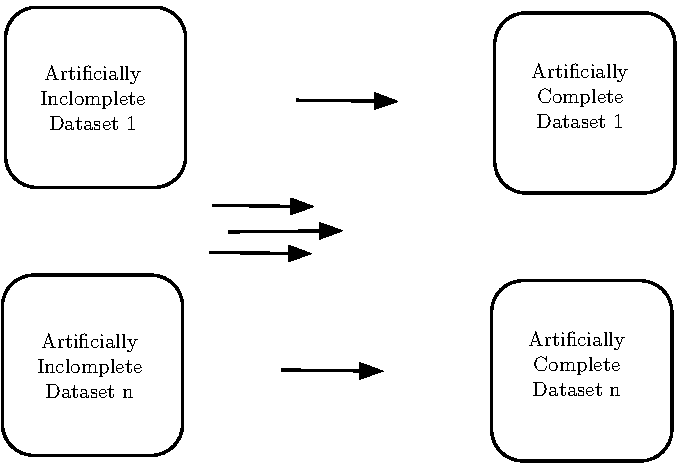
\includegraphics[width=0.35\textwidth]{stage3-2.pdf}
		\end{figure}
		\\
		\indent \textbf{Stage 4: Cluster all Datasets}
		In order to evaluate the effect of an imputation method, by using clustering techniques one can evaluate the distance between all $artComp.i$ and $CC$. By finding the distance between sets of cluster; one can see how close (or far) an imputation method has taken each $artMiss.i$ from the true values (the benchmark $CC$).
		It will now be possible to compare the effect of different imputation methods.

		Thus it is needed to cluster our benchmark dataset $CC$ and all imputed datasets $artComp.i$, $clustCC$ will be the clustering of $CC$ and $clust.i$ will be all clustered $artComp.i$. Note that as with imputing all datasets one needs to make sure the same clustering method with the same parameters are being used on all datasets. This way one can accurately calculate the distances between the clusterings.
		\begin{figure}[!ht]
			\caption{Stage 4}
			\centering
			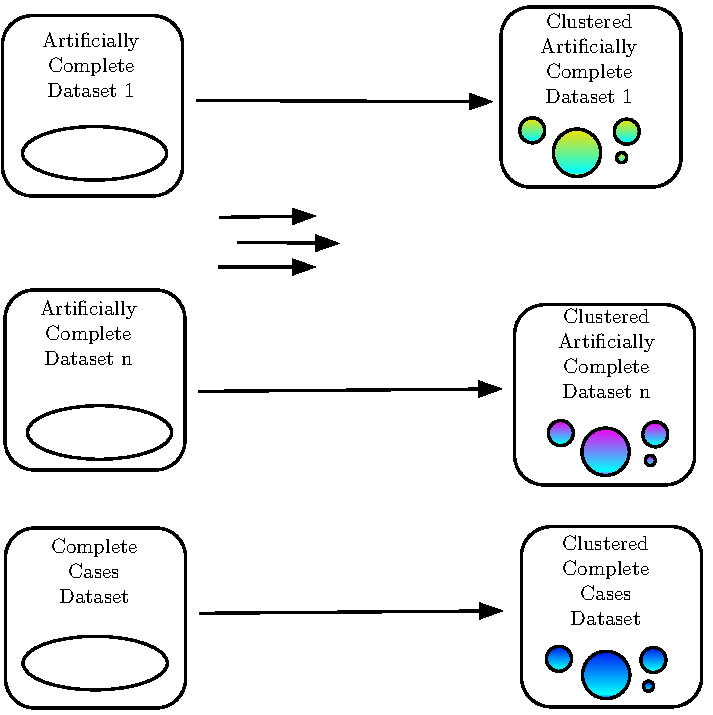
\includegraphics[width=0.35\textwidth]{stage4-2.pdf}
		\end{figure}
		\\
		\indent \textbf{Stage 5: Distance Between Artificial Datasets and Benchmark}
		Finally, calculate the distance between all $clust.i$ and $clustCC$. This will indicate the effect of imputing an incomplete dataset by finding the distance between the clustering of the imputed datasets ($clust.i)$ and the clustering of our benchmark ($clustCC$). The system should output an efficiency indicator to show how far away all $clust.i$ are from $clustCC$; this will be how the user judges whether an imputation method gives correct values or not. Whether the final output describes a successful or efficient imputation method will be subjective. The output should be a normalised result in order to make comparison with other imputation outcomes clearer. The aim is to make it easier for all researchers to see the effect of imputation and feel more comfortable in using data with missing values for analysis.

		It will be up to the researcher to decide whether the imputed values are close enough to represent the truth or whether they are too far to provide fair results from any type of analysis.
		\begin{figure}[!ht]
			\centering
			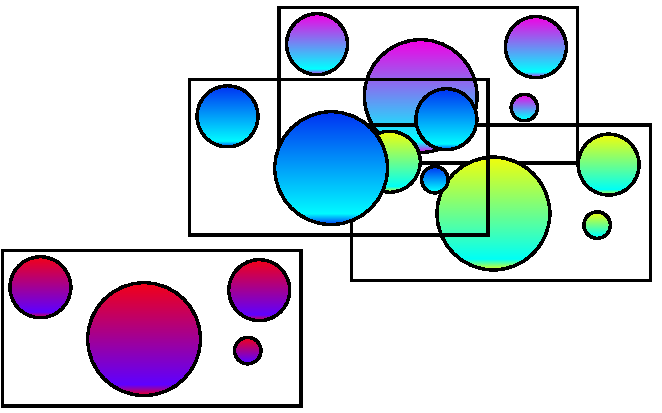
\includegraphics[width=0.35\textwidth]{stage5-2.pdf}
			\caption{Stage 5}
			\label{fig:stage-5}
		\end{figure}

		Figure \ref{fig:stage-5} is a visual representation of what comparing different clustered datasets looks like. Each box contains represents a clustering and contain clusters. Using clustering characteristics, one can compare clustering and evaluate whether clustering A is more similar to clustering B than clustering C is.
	% section proposed_framework (end)

	\section{Preliminary Results} % (fold)
	\label{sec:preliminary_results}
	Our current implementation, called CLEMI (CLustering to Evaluate Multiple Imputation), implemented in R will be published for the public shortly. 

	One of the biggest challenges in this project has been to create a normalised output which can be used to compare different methods. Such outputs can then be used to create a graph of optimal inclusion (how much data should be included for imputation; ignore any records with >90\% missing values). We would like to find out how much missingness can be tolerated without negatively affecting our analysis. 

	The following preliminary results partially show how one can use the clustering characteristics to compare the effect of multiple imputation, we use mean imputation as a reference point \textcolor{red}{I created the mean imputation method in R, not sure how to reference that}. The system created multiple numbers of imputed datasets and after clustering them, we create a table of the averaged cluster characteristics. 

	The characteristics are: the amount of objects in each cluster (clust size), the maximum dissimilarity for each cluster (max-diss), the average dissimilarity for each cluster (avg-diss), the average width for each cluster (avd-width) and the average clusters width for each clustering (avg-widths). 

	For the following tests, the system has created 6 artificial missing datasets by deleting values from the benchmark, it them imputed 1 with mean imputation and 5 with MICE. The system then clusters the benchmark dataset, the mean imputed dataset and all 5 MICE imputed datasets. It then combines the 5 MICE imputed clusterings and outputs the characteristics.
	\\

	Benchmark: Table \ref{benchmark-clust} shows the clustering characteristics for the benchmark dataset, that is the complete cases dataset.\\
		\begin{table}[h!]
		\begin{tabular}{ccc}
		Clust size & max-diss & avg-diss \\
		160 & 5.857 & 2.027 \\
		128 & 3.947 & 1.897 \\
		46 & 3.976 & 2.375 \\
		\end{tabular}
		% \label{benchmark-1}
		% \caption{Benchmark Clustering characteristics}
		% \end{table}
		% \begin{table}[h!]
			\begin{tabular}{c}
				Avg-width for each cluster \\
				0.146 \space \space 0.265 \space \space 0.347 \\
				Avg-widths for all clusters \\
				0.245 \\
			\end{tabular}
		\caption{Benchmark Clustering Characteristics}
		\label{benchmark-clust}
		\end{table}
		\\

	Mean Imputed: Table \ref{mean-clust} shows the clustering characteristics for the mean imputed dataset. \\
		\begin{table}[h!]
		\begin{tabular}{ c c c  }
		Clust size & max-diss & avg-diss \\
		129 & 3.949 & 1.58 \\
		136 & 5.158 & 1.61 \\
		69 & 3.168 & 1.91 \\
		\end{tabular}
		% \label{mean-1}
		% \caption{Mean Clustering characteristics}
		% \end{table}
		% \begin{table}[h!]
			\begin{tabular}{c}
				Avg-width for each cluster \\
				0.0976 \space \space 0.1286 \space \space 0.2294 \\
				Avg-widths for all clusters \\
				0.139, \\
			\end{tabular}
		\caption{Mean Clustering Characteristics}
		\label{mean-clust}
		\end{table}
		\\

	MICE Imputed Average: Table \ref{mice-clust} shows the average cluster characteristics for all the imputed artificially missing datasets, these are created by applying the amount of missingness to the benchmark.  \\
		\begin{table}[h!]
		\begin{tabular}{ c c c  }
		Clust size & max-diss & avg-diss \\
		177 & 5.058 & 2.002 \\
		108 & 3.49 & 2.124 \\
		49 & 3.32 & 2.185 \\
		\end{tabular}
		% \label{mean-1}
		% \caption{Mean Clustering characteristics}
		% \end{table}
		% \begin{table}[h!]
			\begin{tabular}{c}
				Avg-width for each cluster \\
				0.1815 \space \space 0.2035 \space \space 0.3265 \\
				Avg-widths for all clusters \\
				0.217 \\
			\end{tabular}
		\caption{MICE Clustering Characteristics}
		\label{mice-clust}
		\end{table}
		

	From Tables \ref{benchmark-clust}, \ref{mean-clust}, and \ref{mice-clust}, mean imputation created the best clustering out of the three, this is due to the way mean imputation works. It replaces missing values by the average values for that variable, thus replacing all missing values for values which are more likely to be there, this forces all imputed values to be around the centre of every cluster, making the widths smaller and the distance between object also. 

	From these tables we notice that the characteristics from the MICE imputed datasets are closer to the benchmark's than the mean imputed ones are to the benchmarks. The difference between the benchmark clustering avg-clust and MICE clustering avg-clust is only 0.028, compared to the difference between the benchmark clustering avg-clust and mean clustering avg-clust which is 0.106, around 4 times bigger. 

	From these preliminary tests, we are able to see that imputing a dataset with MICE results in a more representative dataset than imputing with the mean. 

	% section preliminary_results (end)

	\section{Discussion} % (fold)
	\label{sec:discussion}
		The purpose of this paper is to set a guideline for the implementation of a system for researchers to use as much of their data as possible for analysis. The aim is to motivate others to solve problems which arise from missing data as well as to provide solutions for all researchers who have similar problems.

		Some work that need to be considered for the implementation are detailed in Sections 6.1 - 4.4:
		\subsection{Outcomes} % (fold)
		\label{sub:outcomes}
			The outcome from this evaluation process should be a number which can be used to compare different imputation methods without any further need to be manipulated. By this we mean that the output should be some normalised number, percentages are used throughout the country, so they could be a good choice. This will make it easier to compare different imputation methods which would normally have incomparable outputs.
		% subsection outcomes (end)

		\subsection{Distance Between Clusterings} % (fold)
		\label{sub:distance_between_datasets}
			In order to evaluate the effect of imputation, we need to see ``how far'' the imputed dataset has travelled from the benchmark. Using clustering, one can view the differences between the clusterings (not individual clusters), the difference between the benchmark clusterings and the imputed data clusterings. 

			Some of the main clustering characteristics which might be useful for this could be, cluster sizes, cluster medoids, average dissimilarities and isolation values to name a few. These are safe choices as they can be used to calculate distance measures between clusterings. 
		% subsection distance_between_datasets (end)

		\subsection{Reference Point} % (fold)
		\label{sub:reference_point}
			Another thing to consider is the use of a reference to evaluate the imputation method. A reference point is needed to determine whether a given imputed dataset can be classified as ``successfully imputed dataset'' or not. One could use a method which is know to be bad, such as mean imputation which can severely distort the distribution for this variable \cite{mean} and use this to see whether the imputation method in question is adequate.

			% Doing this is similar to know whether to wear a jacket or not depending on a given number, if I told you it was 30 outside today, you wouldn't know whether you should wear a jacket or not, but if I told you it's 30 outside and at 0 water freezes, you now have a reference to help you decide. 
		% subsection reference_point (end)

		\subsection{Extra validation} % (fold)
		\label{sub:extra_validation}
			Another possible way to evaluate the effect of imputing a dataset is to create regression models for each dataset (the benchmark, the imputed dataset and the reference dataset) and compare the models. If one created a model for one of the datasets and applies the same technique to the other datasets, the models should reflect any differences between the datasets. By examining how close the model from the imputed dataset is to the benchmark, the user can decide whether the imputation method can be classified as successful or not.
		% subsection extra_validation (end)

	% section discussion (end)

	\section{Conclusion and Future Work} % (fold)
	\label{sec:conclusion}
		Analysis of data with missing values has plagued researchers since the beginning of data collection. Most researchers, especially the less computing inclined, carry out complete case analysis which do not take advantage of all the data available. Doing so may lead to biased analysis or incorrect conclusions. 

		This paper discusses a framework which uses current imputation techniques on data with missing values and evaluate the effect of such imputation. As a result, anyone is be able to create a program which chooses the best imputation method for a given dataset as well as the optimal parameters for a given method. It could also be used to find the limit of missing data which should be allowed to remain (records with a certain amount of missing values will be omitted from analysis).

		This paper can be used as a guideline for anyone who wishes to create a system to evaluate the effect of imputation. This paper also mentions key factors (ability to have any imputation method, change method parameters and output a standardised result) for such a system but has not exhausted them. This paper will be followed by an implementation of this framework, written in R, called CLEMI (Clustering to Evaluate Multiple Imputation). The following paper will explain our implementation choices as well as the testing and evaluation. 
	% section conclusion (end)



	\bibliographystyle{IEEEtran}
	\bibliography{../papers}

\end{document}



A receiver operated characteristic curve will be used to determine the CRL z score with best sensitivity and specificity for outcomes. For asthma severity (measured on ordinal scale of 1-5 and based on treatments prescribed) we will use ordinal logistic regression.



You can look at any cohort study you chose Anthony!  What might be more meaningful is to look at a number of systematic reviews on a topic and then look at the completeness of data within each review.  This will give you 4-5 references which encompass up to 100 original papers.  I attach a SR on asthma aetiology.  You could look for SRs on other non-communicable diseases in  childhood (and ideally the ones you are going to look at, eg obesity, epilepsy, ADHD and diabetes).
 
Best wishes
Steve